\section{证明加密数据的属性}\label{sec:20-2}

在许多应用中,以下情况都会出现。Alice 用 Bob 的公钥加密一个消息 $m$,得到一个密文 $c$。此外,Alice 想向第三方,比如 Charlie(他可以看到 $c$,但看不到 $m$),证明加密后的明文 $m$ 满足某个属性,但不向 Charlie 透露任何关于 $m$ 的其他信息。

一个存在健全的、特殊 HVZK 的 Sigma 协议可以用来解决这类问题。然而,这样的协议并不是一个完整的解决方案。一个问题是,只有 Charlie 诚实地遵循验证协议时,HVZK 属性才能保证不泄露关于 $m$ 的信息。解决这个问题的一个方法就是使用我们在 \ref{subsec:19-6-1} 小节介绍想法,将交互式识别协议变成签名。也就是说,我们不使用实际的验证者来生成随机挑战,而是使用哈希函数来生成挑战。我们将在下一节中详细介绍这种方法。现在,让我们先来看几个有趣而重要的例子,看看我们如何使用 Sigma 协议来证明加密数据的特定属性。

在我们的例子中,简便起见,我们使用 ElGamal 加密方案的乘法变体,我们曾在练习 11.5 中讨论过。该方案利用由 $g\in\mathbb{G}$ 生成的素阶 $q$ 的循环群 $\mathbb{G}$,私钥是随机选择的 $\alpha\in\mathbb{Z}_q$,公钥是 $u:=g^\alpha\in\mathbb{G}$。明文 $m$ 的加密是 $(v,e)\in\mathbb{G}^2$,其中 $v:=g^\beta$,$e:=u^\beta\cdot m$,并且 $\beta$ 也是从 $\mathbb{Z}_q$ 中随机选取的。要用私钥 $\alpha$ 解密 $(v,e)$,我们需要计算 $m:={e}/{v^\alpha}$。正如我们曾在练习 11.5 中要求的那样,可以证明当 $\mathbb{G}$ 满足 DDH 假设时,上述方案是语义安全的。

\begin{example}[明文相等]
假设 Alice 用 Bob 的公钥 $u_0$ 加密了消息 $m$,得到密文 $(v_0,e_0)$。然后 Alice 又用 Bill 的公钥 $u_1$ 加密了同一个消息 $m$,得到了密文 $(v_1,e_1)$。她想让 Charlie 相信两个密文对应的明文相同,但又不透露任何关于明文的信息。比如说,一些协议可能要求 Alice 向 Bob 和 Bill 广播相同的消息。针对这种场景的协议要求在保持消息加密的同时能够证明 Alice 所加密的明文消息确实是相同的。

因此,所以我们希望有一个关系:
$$
\mathcal{R}:=
\bigg\lbrace
\Big(
(\beta_0,\beta_1,m), (u_0,v_0,e_0,u_1,v_1,e_1)
~\Big) :\\
v_0=g^{\beta_0},\;
e_0=u_0^{\beta_0}\cdot m,\;
v_1=g^{\beta_1},\;
e_1=u_1^{\beta_1}\cdot m\,
\bigg\rbrace
$$
上的 Sigma 协议。语言 $L_\mathcal{R}$ 是元组 $(u_0,v_0,e_0,\,u_1,v_1,e_1)$,使得 $(v_0,e_0)$ 和 $(v_1,e_1)$ 对应在公钥 $u_0$ 和 $u_1$ 下加密的同一消息 $m$。

为了设计一个关系 $\mathcal{R}$ 上的有效 Sigma 协议,我们注意到 $(u_0,v_0,e_0,\,u_1,v_1,e_1)\in L_\mathcal{R}$ 就等价于:
$$
v_0=g^{\beta_0},\;
v_1=g^{\beta_1},\;
{e_0}/{e_1}=u_0^{\beta_0}u_1^{-\beta_1},\ 
\text{ for some }\ \beta_0,\beta_1\in\mathbb{Z}_q
$$

基于这一观察,我们可以使用 \ref{subsec:19-5-3} 小节中介绍的通用线性协议实现一个关系 $\mathcal{R}$ 上的 Sigma 协议。具体来说,Alice 需要向 Charlie 证明存在 $\beta_0$ 和 $\beta_1$ 使得方程组:
$$
v_0 =g^{β_0},\;
v_1=g^{\beta_1},\;
{e_0}/{e_1}=u_0^{\beta_0}u_1^{-\beta_1}
$$
成立。这样就得到了一个关系 $\mathcal{R}$ 上的存在健全的、特殊 HVZK 的 Sigma 协议。

请注意,尽管 Alice 在上述协议中没有显式地使用消息 $m$,但 Alice 还是需要知道它,因为她需要同时知道 $\beta_0$ 和 $\beta_1$,其中任何一个都决定了 $m$。
\end{example}

\begin{example}[明文相等2]
考虑上个例子的一个变体。现在 Alice 有两个密文 $(v_0,e_0)$ 和 $(v_1,e_1)$,这两个密文均来自于 Bob 的公钥 $u$ 所加密的相同的明文。不同的地方在于,现在两个密文均对应着使用\emph{相同}公钥加密的相同明文。同样的,Alice 想要向 Charlie 证明这一事实,但又不向他透露其他信息。注意到,如果 $(v_0,e_0)$ 和 $(v_1,e_1)$ 来自相同的明文,那么:
$$
v_0 =g^{\beta_0},\ 
e_0 =u^{\beta_0}·m,\ 
v_1 =g^{\beta_1},\ 
e_1 =u^{\beta_1}·m
$$
其中 $\beta_0,\beta_1\in\mathbb{Z}_q$,$m\in\mathbb{G}$。用第一式除以第三式,第二式除以第四式,我们可以得到:
\begin{equation}\label{eq:20-2}
{v_0}/{v_1}=g^\beta,\;\;
{e_0}/{e_1}=u^\beta
\end{equation}
其中 $\beta:=\beta_0-\beta_1$。此外,不难看出,如果式 \ref{eq:20-2} 对于某个 $\beta\in\mathbb{Z}_q$ 成立,则 $(v_0,e_0)$ 和 $(v_1,e_1)$ 必然来自对相同明文的加密。

因此,Alice 需要做的就是让 Charlie 相信存在满足式 \ref{eq:20-2} 的 $\beta$。为此,她可以使用 \ref{subsec:19-5-3} 小节介绍的通用线性协议。在本例的场景下,它其实就是证明 $(u,{v_0}/{v_1},{e_0}/{e_1})$ 是一个 DH 三元组的 Chaum-Pedersen 协议(见 \ref{subsec:19-5-2} 小节)。

需要注意的是,为了证明 $(v_0,e_0)$ 和 $(v_1,e_1)$ 加密了相同的消息,Alice 只需要知道满足上式的 $\beta$,她并不需要知道明文消息 $m$ 本身。特别地,Alice 不需要是产生这些密文的一方。事实上,她可以从其他方收到密文 $(v_0,e_0)$,然后通过计算 $v_1:=v_0\cdot g^\beta$ 和 $e_1:=e_0\cdot u^\beta$ 为她选择的 $\beta$ 创建同一消息 $m$ 的新密文 $(v_1,e_1)$。一些匿名服务就能执行类似的功能,他们能够利用这个协议对一个加密消息进行重加密。这个协议可以用来确保这一过程被正确完成。
\end{example}

\begin{example}[加密后的比特]\label{exmp:20-3}
为了加密一个比特 $b\in\{0,1\}$,比较方便的做法是将 $b$ 编码为群元素 $g^b\in\mathbb{G}$,然后用乘性 ElGamal 对 $g^b$ 进行加密。因此,假设 Alice 以这种方式用 Bob 的公钥 $u$ 对比特 $b$ 进行加密,产生一个密文 $(v,e)=(g^\beta,u^\beta\cdot{g^b})$。她想让 Charlie 相信 $(v,e)$ 确实是由 Bob 的公钥加密一个比特得到的(而不是加密其他的什么东西,比如 $g^{17}$),而又不向 Charlie 透露任何其他信息。

因此,我们希望有一个关系:
$$
\mathcal{R}:=
\bigg\lbrace
\Big(
(b,\beta),(u,v,e)
\Big):
v=g^\beta,\;
e=u^\beta\cdot g^b,\;
b\in\{0,1\}\;
\bigg\rbrace
$$
上的 Sigma 协议。与此关系相对应的语言 $L_{\mathcal R}$ 是一个元组 $(u,v,e)$,满足 $(v,e)$ 是用公钥 $u$ 加密一个比特得到的。

我们的 $\mathcal{R}$ 上的 Sigma 协议基于下面的观察,即$(u,v,e)\in L_{\mathcal R}$等价于:
$$
\text{either }
(u,v,e)
\text{ or }
(u,v,{e}/{g})
\text{ is a DH-triple}
$$
\ref{subsec:19-5-2} 中介绍的 Chaum-Pedersen 协议允许一方证明一个给定的三元组是 DH 三元组。我们把它与 \ref{subsec:19-7-2} 中介绍的 OR 证明构造结合起来。这为我们提供了一个关系:
$$
\mathcal{R}':=
\bigg\lbrace
\Big(
(b,\beta),\;((u_0,v_0,w_0),\;(u_1,v_1,w_1))
\Big):
v_b=g^\beta,~
w_b=u_b^\beta\;
\bigg\rbrace
$$
上的 Sigma 协议。如果 $(u_0,v_0,w_0)$,$(u_1,v_1,w_1)$ 中至少有一个是 DH 三元组,则语句 $((u_0,v_0,w_0),(u_1,v_1,w_1))$ 就在 $L_{\mathcal{R}'}$ 中。于是,我们有:
$$
(u,v,e)\in L_{\mathcal R}\ \iff\ 
\Big((u,v,e),(u,v,{e}/{g})\Big)\in L_{\mathcal R'}
$$
因此,为了让 Alice 向 Charlie 证明 $(u,v,e)\in L_{\mathcal{R}}$,可以使用陈述 $((u,v,e),(u,v,{e}/{g}))$ 和见证 $(b,\beta)$ 运行一个 $\mathcal{R}'$ 上的 Sigma 协议。完整起见,我们在图 \ref{fig:20-1} 中展示了完整的 $\mathcal R$ 上的 Sigma 协议。在证明者逻辑的第一行,证明者为其知道的见证启动证明过程,第二和第三行为其不知道的见证运行 HVZK 模拟器。由此产生的 $\mathcal R$ 上的 Sigma 协议是存在健全的,并且是特殊 HVZK 的。

\begin{figure}
  \centering
  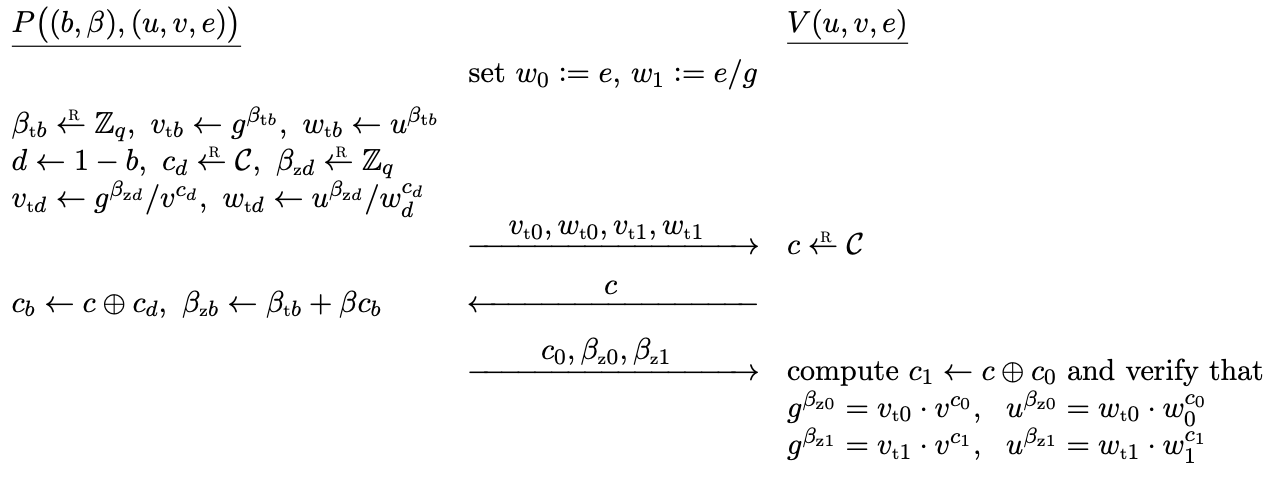
\includegraphics[width=0.85\linewidth]{figures/chapter20/fig1.png}
  \caption{用于加密比特的 Sigma 协议}
  \label{fig:20-1}
\end{figure}

正如练习 20.6 将要说明的,该协议可以泛化为证明一个密文 $(v,e)$ 在 $B>2$ 的情况下加密了一个值 $0\leq b < B$。该协议的交互记录随 $B$ 的增大线性增长,因此只适用于相对较小的 $B$。我们会在 \ref{subsec:20-4-1} 小节介绍如何处理 $B$ 较大的情况。
\end{example}

\begin{example}[加密后的 DH 三元组]\label{exmp:20-4}
假设 Alice 有一个 DH 三元组 $(g^{\gamma_1},g^{\gamma_2},g^{\gamma_3})$,其中 $\gamma_3=\gamma_1\gamma_2$。她使用 Bob 的公钥 $u$ 对每个元素进行加密,生成了三条密文 $(v_1,e_1)$,$(v_2,e_2)$,$(v_3,e_3)$,其中:
\begin{equation}\label{eq:20-3}
v_i=g^{\beta_i},\;
e_i=u^{\beta_i}g^{\gamma_i}\;\;
(i = 1,2,3)
\end{equation}
她把这些密文交给 Charlie,并想让他相信这些密文确实是对一个 DH 三元组的加密,但又不透露任何其他信息。

因此,我们希望有一个关系:
$$
\mathcal R:=
\bigg\lbrace
\Big((\beta_1,\beta_2,\beta_3,\gamma_1,\gamma_2,\gamma_3),(u,v_1,e_1,v_2,e_2,v_3,e_3)\Big):\\
v_i=g^{\beta_i},\;
e_i=u^{\beta_i}g^{\gamma_i}\,(i=1,2,3),\;
\gamma_3=\gamma_1\gamma2
\bigg\rbrace
$$
上的 Sigma 协议。相应的语言 $L_{\mathcal R}$ 是满足密文 $(v_1,e_1)$,$(v_2,e_2)$,$(v_3,e_3)$ 是由公钥 $u$ 加密一个 DH 三元组得到的元组 $(u,\;v_1,e_1,\;v_2,e_2,\;v_3,e_3)$。

虽然由于条件 $\gamma_3=\gamma_1\gamma_2$,关系 $\mathcal R$ 本质上是非线性的,但我们还是可以使用 \ref{subsec:19-5-3} 中介绍的通用线性协议为 $\mathcal R$ 设计一个 Sigma 协议。其基本思想是,Alice 向 Charlie 证明,存在$\beta_1$、$\beta_3$、$\gamma_1$ 和 $\tau$满足方程组:
\begin{equation}\label{eq:20-4}
v_1=g^{\beta_1},~~
e_1=u^{\beta_1}g^{\gamma_1},~~
v_3=g^{\beta_3},~~
v_2^{\gamma_1}=g^\tau,~~
e^{\gamma_1}u^{\beta_3}=e_3u^\tau
\end{equation}

为了证明这一点,我们声称 $(u,v_1,e_1,v_2,e_2,v_3,e_3)\in L_{\mathcal R}$ 成立当且仅当存在能够满足式 \ref{eq:20-4} 的 $\beta_1,\beta_3,\gamma_1,\tau$。注意到,密文 $(v_1,e_1)$,$(v_2,e_2)$,$(v_3,e_3)$ 唯一决定了 $\beta_i$ 和满足式 \ref{eq:20-3} 的 $\gamma_i$。$\beta_1$,$\beta_3$ 和 $\gamma_1$ 也是满足式 \ref{eq:20-4} 中前三个等式的唯一值。式 \ref{eq:20-4} 中的第四个方程可以通过令 $\tau:=\gamma_1\beta_2$ 而得到唯一的满足。因此,剩下的工作就是考虑式 \ref{eq:20-4} 中最后一个方程,其等号左边为:
$$
e^{\gamma_1}u^{\beta_3}=(u^{\beta_2}g^{\gamma_2})^{\gamma_1}u^{\beta_3}=u^{\beta_3+\tau}g^{\gamma_1\gamma_2}
$$
而等号右边为:
$$
e_3u^\tau=(u^{\beta_3}g^{\gamma_3})u^\tau =u^{\beta_3+\tau}g^{\gamma_3}
$$
因此,当且仅当 $\gamma_1\gamma_2=\gamma_3$ 时,该方程成立。这就证明了我们的声称。

这样,我们就得到了 $\mathcal R$ 上的 Sigma 协议。为了运行该协议,Alice 使用见证 $(\beta_1,\beta_3,\gamma_1,\tau:= \gamma_1\beta_2)$ 运行式 \ref{eq:20-4} 的通用线性协议。该协议的正确性、存在健全性和特殊 HVZK 性都来自于通用线性协议的相应属性。
\end{example}

\begin{example}[加密后的比特 2]\label{exmp:20-5}
利用上一个例子的思路,我们可以得到用于例 \ref{exmp:20-3} 中加密比特问题的另一个 Sigma 协议。

如果 Alice 想向 Charlie 证明密文 $(v,e)$ 形如 $v=g^\beta$,$e=u^\beta g^b$,其中 $b=\{0,1\}$,她只需要说明 $b^2=b$,因为 $b\in\mathbb{Z}_q$ 中满足 $b^2=b$ 的就只有 $b=0$ 或者 $b=1$。

因此,使用通用线性协议,Alice 只要向 Charlie 证明存在 $b,\beta,\tau(=\beta b)$ 满足方程组:
$$
v=g^\beta,~~
e=u^\beta g^b,~~
v^b=g^\tau,~~
e^b=u^\tau g^b
$$
读者可以自行验证这是否能够产生针对例 \ref{exmp:20-3} 中关系 $\mathcal R$ 的一个存在健全的、特殊 HVZK 的 Sigma 协议。所得到的协议与例 \ref{exmp:20-3} 中的加密比特协议具有类似的性能表现。

这个协议可以推广到向 Charlie 证明,一个密文 $(v,e)$ 来自对值 $0\leq b < B$ 的加密,其中 $B>2$。这种推广使用到了下一个例子中将要介绍的 Sigma 协议,用于向 Charlie 证明 $b$ 满足多项式关系$b(b-1)(b-2)\cdots(b-(B-1))=0$。该关系意味着 $0\leq b < B$。该协议的交互记录同样随 $B$ 的增大而线性增长,因此也只适用于相对较小的 $B$。
\end{example}

\begin{example}[多项式关系]\label{exmp:20-6}
我们可以进一步扩展例 \ref{exmp:20-4} 的想法。假设 Alice 用 Bob 的公钥 $u$ 生成两个密文 $(v,e)$ 和 $(v',e')$,第一个密文来自对群元素 $g^\gamma$ 的加密,第二个则来自 $g^{\gamma'}$。Alice 想让 Charlie 相信,对于某个特定的多项式 $f(x)=\sum_{i=0}^d\lambda_ix^i$,有 $\gamma'=f(\gamma)$。我们将假设多项式 $f(x)$ 的阶 $d$ 和系数 $\lambda_0,\dots,\lambda_d$ 都是固定且公开的值(即为常数或者系统参数)。

因此,我们想要一个关系:
$$
\mathcal R=
\bigg\lbrace
\Big((\beta,\gamma,\beta',\gamma'),(u,v,e,v',e')\Big):
v=g^\beta,\;
e=u^\beta\cdot g^\gamma,\;
v'=g^{\beta'},\;
e'=u^{\beta'}\cdot g^{\gamma'},\;
\gamma'=f(\gamma)
\bigg\rbrace
$$
上的 Sigma 协议。

为了得到 $\mathcal R$ 上的 Sigma 协议,Alice 和 Charlie 使用通用线性协议,其中 Alice 向 Charlie 证明,存在:
$$
\beta,~~~
\gamma_1,\dots,\gamma_d,~~~
\tau_1,\dots,\tau_{d-1},~~~
\beta',~
\gamma'
$$
满足方程组:
\begin{equation*}
\begin{aligned}
& v=g^\beta,\;
e=u^\beta g^{\gamma_1},\;
v'=g^{\beta'},\;
e'=u^{\beta'}g^{\gamma'},\;
\gamma'=\lambda_0+\lambda_1\gamma_1+\cdots+\lambda_d\gamma_d,\\
& v^{\gamma_i}=g^{\tau_i},\;
e^{\gamma_i}=u^{\tau_i}g^{\gamma_{i+1}}\;\;\;
(i=1,\dots,d-1)
\end{aligned}
\end{equation*}
请注意,这里我们使用的是通用线性协议的推广版本,它能够处理 $\mathbb G$ 和 $\mathbb{Z}_q$ 上的方程(见定理 \ref{theo:19-11} 之后的讨论)。Alice 使用 $\gamma_i:=\gamma^i,~~i=1,\dots,d$ 和 $\tau_i:=\beta\gamma^i,~~i=1,\dots,d-1$ 运行该协议。读者可以证明,这些实际上是满足这个方程组的唯一取值。通过一个简单的归纳论证可以很容易地证明这一点。由此可见,所得到的 Sigma 协议是一个关系 $\mathcal R$ 上存在健全的,特殊 HVZK 的Sigma 协议。
\end{example}

以上的例子展示了\emph{语言规约}的概念。一般来说,这种从 $\mathcal{R}\subseteq\mathcal{X}\times\mathcal{Y}$ 到 $\mathcal{R}'\subseteq\mathcal{X}'\times\mathcal{Y}'$ 的规约是一对可有效计算的映射 $f:\mathcal{X}\times\mathcal{Y}\to\mathcal{X}'$ 和 $g:\mathcal{Y}\to\mathcal{Y}'$,使得:
\begin{enumerate}[(i)]
	\item 对于所有 $(x,y)\in\mathcal{R}$ 都有 $(f(x,y),g(y))\in\mathcal{R}'$ 成立,并且
	\item 对于所有 $y\in\mathcal{Y}$,$g(y)\in L_{\mathcal{R}'}\; \Longrightarrow\; y\in L_{\mathcal R}$。
\end{enumerate}
利用这样的规约,我们就可以利用 $\mathcal{R}'$ 上的 Sigma 协议 $\Pi'$ 来构造一个 $\mathcal{R}$ 上的 Sigma 协议 $\Pi$。上面的第一个条件能够确保 $\Pi$ 能够从 $\Pi'$ 处继承正确性和特殊 HVZK 性,第二个条件确保 $\Pi$ 能够从 $\Pi'$ 处继承存在健全性。注意,知识可靠性不一定需要继承。也就是说,我们不要求可以从 $g(y)$ 的见证中恢复 $y$ 的见证。在上述几乎所有的例子中,关系 $\mathcal{R}'$ 都是通用线性关系的特例。唯一的例外是例 \ref{exmp:20-3},其关系 $\mathcal{R}'$ 来自 OR 证明构造。

\subsection{一种用于非线性关系的通用协议}\label{subsec:20-2-1}

在上面的几个例子中,我们可以看到,通用线性协议可以用于证明某些非线性关系。我们下面将展示更加通用的情况。正如我们将要看到的,例 \ref{exmp:20-6} 中的多项式求值协议可以很容易地推导出这种构造的一个特例。同样的通用构造也可以用来推导出针对例 \ref{exmp:20-4} 和例 \ref{exmp:20-4} 中的问题的协议;然而,所得到的协议不会像这两个例子中的协议那样高效。

与往常一样,令 $\mathbb{G}$ 是一个由 $g\in\mathbb{G}$ 生成的素阶 $q$ 的循环群。考虑 \ref{subsec:19-5-3} 小节中介绍的通用线性协议,该协议适用于形如式 \ref{eq:19-13} 所描述的公式 $\phi$。假设我们现在也允许 $\phi$ 中存在形如 $x_i=x_j\cdot x_k$ 的非线性方程。为了这个构造仍然有效,我们要求对于每个这样的非线性方程,$\phi$ 中还需要包含形如下面这样的两个辅助方程:
\begin{equation}\label{eq:20-5}
v=g^{x_\ell},\;\;
e=u^{x_\ell}g^{x_j}
\end{equation}
其中 $u$,$v$ 和 $e$ 都是群 $\mathbb{G}$ 中的元素,而 $x_\ell$ 是某个变量。为了简单起见,我们假设在对 $\phi$ 的描述中,存在从每个非线性方程到对应辅助方程的指针。

我们可以将这样的公式 $\phi$ 转化为可以使用通用线性协议处理的方程 $\phi'$,方法如下。对于 $\phi$ 中的每个非线性方程 $x_i=x_j\cdot x_k$ 以及式 \ref{eq:20-5} 中相应的辅助方程,我们引入一个临时变量 $t$,并将非线性方程 $x_i=x_j\cdot x_k$ 替换为下面的一对方程:
\begin{equation}\label{eq:20-6}
v^{x_k}=g^t,~~
e^{x_t}=u^th^{x_i}
\end{equation}

这种变换的结果就是一个可以用通用线性协议处理的方程 $\phi'$。用于 $\phi$ 的 Sigma 协议的工作原理如下。证明者和验证者都可以将 $\phi$ 转化为 $\phi'$。假设证明者有变量 $(x_1,\dots,x_n)$ 的一个赋值 $(\alpha_1,\dots,\alpha_n)$,该赋值能够使得 $\phi$ 的值为 $\mathsf{true}$。那么对于 $\phi$ 中的每个非线性方程 $x_i=x_j\cdot x_k$,证明者为式 \ref{eq:20-6} 中的临时变量 $t$ 赋值 $\alpha_k\alpha_\ell$,然后用这个扩展赋值与验证者一起运行 $\phi'$ 的通用线性协议。

读者可以验证,这种变换得到的 Sigma 协议是特殊 HVZK 的,并且为关系 \ref{eq:19-14} 提供知识健全性,其中方程 $\phi$ 现在被允许具有上述的非线性形式。

\begin{snote}[多项式计算.]
例 \ref{exmp:20-6} 中的协议可以用这种转换方式导出。Alice 向 Charlie 证明,存在:
$$
\beta,~~
\gamma_1,\dots,\gamma_d,~~
\beta',~
\gamma'
$$
满足方程组:
\begin{equation*}
\begin{aligned}
& v=g^\beta,~~
e=u^\beta g^{\gamma_1},~~
v'=g^{\beta'},~~
e'=u^{\beta'}g^{\gamma'},~~
\gamma'=\lambda_0+\lambda_1\gamma_1+\cdots+\lambda_d\gamma_d,\\
& \gamma_{i+1}=\gamma_1\cdot\gamma_i~~~(i=1,\dots,d-1)
\end{aligned}
\end{equation*}
读者可以自行验证,从非线性到线性的变换能够将每个方程 $\gamma_{i+1}=\gamma_1\cdot\gamma_i$ 转换为一对方程 $v^{\gamma_i}=g^{\tau_i}$ 和 $e^{\gamma_i}=u^{\tau_i}g^{\gamma_{i+1}}$。
\end{snote}

\begin{snote}[加密后的比特.]
例 \ref{exmp:20-5} 中的协议也可以用这种变换得出。Alice 向 Charlie 证明存在 $b$ 和 $\beta$ 使得:
$$
v=g^\beta,\;
e=u^\beta g^b,\;
b=b\cdot b
$$
成立。读者可以自行证明,从非线性到线性的变换能够得出例 \ref{exmp:20-5} 中的协议。
\end{snote}

\begin{snote}[加密后的 DH 三元组.]

我们也可以尝试使用这种技术来设计例 \ref{exmp:20-4} 中的协议。最明显的方法是让 Alice 向 Charlie 证明,存在:
$$
\beta_1,\beta_2,\beta_3,~~~~
\gamma_1,\gamma_2,\gamma_3
$$
使得:
$$
v_i=g^{\beta_i},\;
e_i=u^{\beta_i}g^{\gamma_i}~~(i=1,2,3),\;
\gamma_3=\gamma_1\gamma_2
$$
成立。我们可以将这个方程组插入上述从非线性到线性的变换中。这样做是可行的,但得到的协议不会像例 \ref{exmp:20-4} 中的协议那样高效。
\end{snote}

\begin{snote}[去除对非线性方程的约束.]
虽然我们的通用变换相当有用,但它仍然受到一定的限制。事实上,我们要求对于每个非线性方程 $x_i=x_j\cdot x_k$,方程组还必须包括描述使用乘性 ElGamal 加密 $x_j$ 或 $x_k$ 的方程。稍后,在 \ref{subsec:20-4-3} 小节中,我们将看到,如果我们愿意使用相对较弱(但仍然有用)的 HVZK 形式(或较弱的知识健全性形式,见练习 20.5),我们就可以去掉这一要求。
\end{snote}